\chapter{ハール分布と量子回路の表現力}\label{chap:haar}
変分量子アルゴリズムにおいては、しばしば、パラメーターの初期値がランダムに選ばれ、それがバレンプラトーと関係することを前章で述べた。ユニタリ群における一様なランダムネスを考える場合、ハール分布やユニタリデザインという概念が重要になる。後の\ref{chap:upper-bound}, \ref{chap:lower-bound}~章の解析においても、これらの概念に基づいて解析を行う。よって、この章においては、ハール分布やユニタリデザインの定義から始め、それらの性質や関連する定理、更に量子回路の表現力と呼ばれる量について説明する。
\ref{sec:haar-random}~節では、ハール分布とそれに関する積分の公式について説明する。
\ref{sec:unitary-t-design}~節でユニタリ $t$--デザインというユニタリの集合に関する性質について説明する。
\ref{sec:expressibility}~節では、量子回路の表現力について説明する。

\section{ハール分布}\label{sec:haar-random}
ハール分布(測度)とはコンパクト群上の一様分布であり、ユニタリ群上のハール分布 $\mu_{\Haar}$ は、ユニタリ群 $\calU(d)$ 上のユニタリ不変な測度であって、以下の性質を満たすものである。
\begin{align}
    \mu_{\Haar}(\calU(d)) = \const,\;\;
    \mu_{\Haar}(g\bbU) = \mu_{\Haar}(\bbU g) = \mu_{\Haar}(\bbU),\,\,\forall g\in \calU(d),\;\;
    \forall \bbU\subset \calU(d)
\end{align}
ここでは確率分布を考えるため $\mu_{\Haar}(\calU(d)) = 1$ とする。
ハールランダムなユニタリ $U$ とは、ハール分布 $\mu_{\Haar}$ からサンプリングされたユニタリ $U$ のことを指す。

$2\times 2$ 次元のハールランダムなユニタリをサンプリングして $\ket{0}$ に作用させると、それらの状態は、図~\ref{fig:haar-1qubit}のようにブロッホ球面上で一様に分布する。
\begin{figure}[H]
    \centering
    \includegraphics[width=10cm]{haar-sampling.pdf}
    \caption{ブロッホ球面上でのハール分布}
    \label{fig:haar-1qubit}
\end{figure}

% \subsection{ハール分布の積分公式}
ユニタリ群上のハール分布においては、次のような積分公式が成り立つ。
\begin{screen}
    \begin{theorem}
        ハール分布に従うユニタリ $W$ に関する積分は以下のように計算できる。
        \begin{align}
            \int_{\calU(d)} d\mu_{\Haar}(W)\, w_{\bs{i},\bs{j}}
            w_{\bs{p},\bs{q}}^*
            &= \frac{\delta_{\bs{i},\bs{p}}\delta_{\bs{j},\bs{q}}}{d} \label{eq:haar-int-1}\\
            % 
            \int_{\calU(d)} d\mu_{\Haar}(W)\, w_{\bs{i}_1,\bs{j}_1}
            w_{\bs{i}_2,\bs{j}_2}
            w_{\bs{i}_1^\prime,\bs{j}_1^\prime}^*
            w_{\bs{i}_2^\prime,\bs{j}_2^\prime}^*
            &= \frac{1}{d^2-1}
            (\delta_{\bs{i}_1,\bs{i}_1^\prime}\delta_{\bs{i}_2,\bs{i}_2^\prime}
            \delta_{\bs{j}_1,\bs{j}_1^\prime}\delta_{\bs{j}_2,\bs{j}_2^\prime}
            +\delta_{\bs{i}_1,\bs{i}_2^\prime}\delta_{\bs{i}_2,\bs{i}_1^\prime}
            \delta_{\bs{j}_1,\bs{j}_2^\prime}\delta_{\bs{j}_2,\bs{j}_1^\prime}) \nonumber\\
            &- \frac{1}{d(d^2-1)}
            (\delta_{\bs{i}_1,\bs{i}_1^\prime}\delta_{\bs{i}_2,\bs{i}_2^\prime}
            \delta_{\bs{j}_1,\bs{j}_2^\prime}\delta_{\bs{j}_2,\bs{j}_1^\prime}
            +\delta_{\bs{i}_1,\bs{i}_2^\prime}\delta_{\bs{i}_2,\bs{i}_1^\prime}
            \delta_{\bs{j}_1,\bs{j}_1^\prime}\delta_{\bs{j}_2,\bs{j}_2^\prime}) \label{eq:haar-int-2}
        \end{align}
    \end{theorem}
\end{screen}

たとえば、公式~\eqref{eq:haar-int-1} を用いると、次のような積分を計算することができる。
\begin{align}
    \int_{\calU(d)} d\mu_{\Haar}(W)\, |\ev{W}{\bs{0}}|^2
    &= \int_{\calU(d)} d\mu_{\Haar}(W)\, w_{\bs{0},\bs{0}}\,w_{\bs{0},\bs{0}}^*
    = \frac{1}{d}
\end{align}

さらに、公式~\eqref{eq:haar-int-2} を用いることで、次の公式を導くことができる。
\begin{align}\label{eq:haar-int-5}
    \int_{\calU(d)} d\mu_{\Haar}(W)\, \Tr[WAW\dg B]\Tr[WCW\dg D]
    &= \frac{1}{d^2-1}
    (\Tr[A]\Tr[B]\Tr[C]\Tr[D] + \Tr[AC]\Tr[BD]) \nonumber\\
    &- \frac{1}{d(d^2-1)}
    (\Tr[AC]\Tr[B]\Tr[D] + \Tr[A]\Tr[C]\Tr[BD])
\end{align}
\begin{align}\label{eq:haar-int-6}
    \int_{\calU(d)} d\mu_{\Haar}(W)\, \Tr[AW\otn{2}B(W\dg)\otn{2}]
    &= \frac{1}{d^2-1}(\Tr[A]\Tr[B] + \Tr[A\,\SWAP]\Tr[B\,\SWAP]) \nonumber\\
    &- \frac{1}{d(d^2-1)}(\Tr[A\,\SWAP]\Tr[B] + \Tr[A]\Tr[B\,\SWAP])
\end{align}
ただし、$\SWAP = \sum_{i,j=1}^d \ket{ij}\bra{ji}$ である。証明は、論文~\cite{cerezo2021cost}の Supplementary Note 1 を参照。


これらの公式とテンソルネットワークによる記法を組み合わせることで、ハール分布に関する積分を行列の脚の繋ぎ替えたものの和として表現することができる。テンソルネットワークとは、大きな量子状態を効率的に表現するための方法である。以下に、必要なテンソルネットワークの記法を示す。

\begin{figure}[H]
    \centering
    \begin{tikzpicture}[scale=1]
        % Vector
        % Define the nodes
        \node[draw, rectangle] (v) at (0,0) {{\LARGE $v$}};
        % Connect the nodes
        \draw (v) -- (-2, 0) node[left] {$i$};
        
        % Matrix
        % Define the nodes
        \node[draw, rectangle] (A) at (4,0) {{\LARGE $A$}};
        % Connect the nodes
        \draw (A) -- (2, 0) node[left] {$j$};
        \draw (A) -- (6, 0) node[right] {$k$};
    \end{tikzpicture}
    \caption{べクトルと行列}
\end{figure}

\begin{figure}[H]
    \centering
    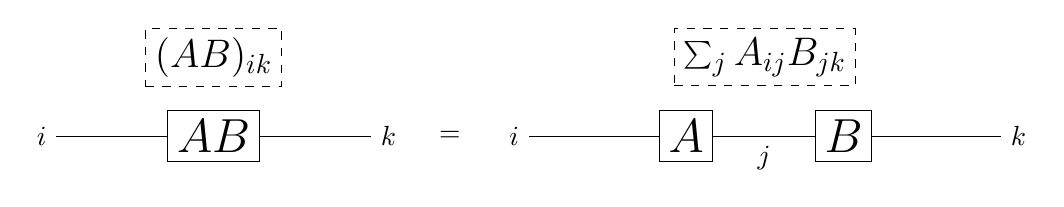
\begin{tikzpicture}[scale=1]
        % Define the nodes
        \node[draw,rectangle]        (AB)  at (-4,0) {{\LARGE $AB$}};
        \node[draw,rectangle,dashed] (eq1) at (-4,1) {{\Large $(AB)_{ik}$}};
        \node[draw,rectangle]        (A)   at (2,0) {{\LARGE $A$}};
        \node[draw,rectangle]        (B)   at (4,0) {{\LARGE $B$}};
        \node[draw,rectangle,dashed] (eq2) at (3,1) {{\Large $\sum_j A_{ij}B_{jk}$}};
        % Connect the nodes
        \draw (AB) -- (-6, 0) node[left] {$i$};
        \draw (AB) -- (-2,0) node[right] {$k$};
        \draw (-1,0) node {$=$};
        \draw (A) -- (0, 0) node[left] {$i$};
        \draw (A) -- (B) node[midway, below] {$j$};
        \draw (B) -- (6, 0) node[right] {$k$};
    \end{tikzpicture}
    \caption{行列の積}
\end{figure}


\begin{figure}[H]
    \centering
    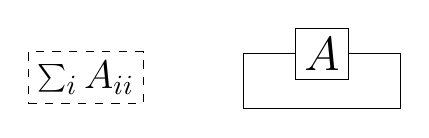
\begin{tikzpicture}[scale=1]
        % Define the nodes for trace
        \node[draw,rectangle]        (A)  at (0,0) {{\LARGE $A$}};
        \node[draw,rectangle,dashed] (eq3) at (-3,-0.3) {{\Large $\sum_i A_{ii}$}};
        % Connect the nodes for trace
        \draw (A.west) -- (-1,0) -- (-1,-0.7) -- (1,-0.7) -- (1,0) -- (A.east);
    \end{tikzpicture}
    \caption{トレース}
\end{figure}

\begin{comment}
\begin{figure}[H]
    \centering
    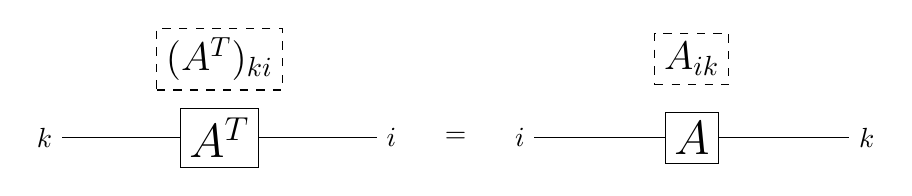
\begin{tikzpicture}[scale=1]
        % Define the nodes for transpose
        \node[draw,rectangle]        (AT)  at (-4,0) {{\LARGE $A^T$}};
        \node[draw,rectangle,dashed] (eq1) at (-4,1) {{\Large $(A^T)_{ki}$}};
        \node[draw,rectangle]        (A)   at (2,0) {{\LARGE $A$}};
        \node[draw,rectangle,dashed] (eq2) at (2,1) {{\Large $A_{ik}$}};
        % Connect the nodes for transpose
        \draw (AT) -- (-6, 0) node[left] {$k$};
        \draw (AT) -- (-2,0) node[right] {$i$};
        \draw (-1,0) node {$=$};
        \draw (A) -- (0, 0) node[left] {$i$};
        \draw (A) -- (4,0) node[right] {$k$};
    \end{tikzpicture}
    \caption{行列の転置}
\end{figure}

\begin{figure}[H]
    \centering
    \includegraphics[width=10cm]{tensor-mat@vec.png}
    \caption{}
\end{figure}

\begin{figure}[H]
    \centering
    \includegraphics[width=14cm]{tensor-vec-t.png}
    \caption{}
\end{figure}

\begin{figure}[H]
    \centering
    \includegraphics[width=10cm]{tensor-mat-t.png}
    \caption{}
\end{figure}
\end{comment}


例えば、公式~\eqref{eq:haar-int-1}を用いて、次の積分公式を示せる。
\begin{align}\label{eq:haar-int-3}
    \int_{\calU(d)} d\mu_{\Haar}(U)\; AUBU\dg C = \frac{\Tr[B]AC}{d}
\end{align}
テンソルネットワークによる記法を用いると、図~\ref{fig:haar-int-3}のように表現することができる。

\begin{figure}[H]
    \centering
    \includegraphics[width=14cm]{haar-int.pdf}
    \caption{公式~\eqref{eq:haar-int-3}に対応するテンソルネットワーク}
    \label{fig:haar-int-3}
\end{figure}

また、公式~\eqref{eq:haar-int-2}を用いて、次の積分公式を示せる。
\begin{align}\label{eq:haar-int-4}
    \int_{\calU(d)} d\mu_{\Haar}(U)\;AUBU\dg CUDU\dg E &= \frac{1}{d^2-1}(\Tr[B]\Tr[D]ACE + \Tr[BD]\Tr[C]AE) \nonumber\\
    &\quad - \frac{1}{d(d^2-1)}(\Tr[BD]ACE + \Tr[B]\Tr[C]\Tr[D]AE)
\end{align}
テンソルネットワークによる記法を用いると、図~\ref{fig:haar-int-4}のように表現することができる。

\begin{figure}[H]
    \centering
    \includegraphics[width=14cm]{haar-int-2.pdf}
    \caption{公式~\eqref{eq:haar-int-4}に対応するテンソルネットワーク}
    \label{fig:haar-int-4}
\end{figure}


% \begin{align}
%     \int_{\calU(d)} d\mu_{\Haar}(W)\, 
%     \Tr[WAW\dg B]
%     &= \frac{\Tr[A]\Tr[B]}{d}
% \end{align}

% \begin{align}
%     \int_{\calU(d)} d\mu_{\Haar}(W)\, \Tr[WAW\dg BWCW\dg D]
%     &= \frac{1}{d^2-1}
%     (\Tr[A]\Tr[C]\Tr[BD] + \Tr[AC]\Tr[B]\Tr[D]) \nonumber\\
%     &- \frac{1}{d(d^2-1)}
%     (\Tr[AC]\Tr[BD] + \Tr[A]\Tr[B]\Tr[C]\Tr[D])
% \end{align}



\section{ユニタリ $t$--デザイン}\label{sec:unitary-t-design}
ユニタリ $t$--デザインとは、ユニタリの集合に関する性質の一つであり、次のように定義される。
\begin{screen}
    \begin{definition}
        $P_{t,t}(U)$ は、ユニタリ $U$ と $U\dg$ のそれぞれの成分に関して最大次数 $t$ の斉次多項式とする。$K$ 個のユニタリの集合 $\{U_k\}$ が以下の条件を満たすとき、この集合はユニタリ $t$--デザインを成すという。
        \begin{align}
            \frac{1}{K} \sum_{k=1}^{K} P_{t,t}(U_k) = \int_{\calU(d)} P_{t,t} (U) d\mu_{\Haar}(U)
        \end{align}
        ここで、$d\mu_{\Haar}$ はハール分布である。
    \end{definition}
\end{screen}
すなわち、ユニタリ $t$--デザインとは、ユニタリの集合に関する斉次多項式 $P_{t,t}(U)$ の平均値が、ユニタリ群上のハール分布に関する積分と厳密に等しいような性質のことである。
ユニタリ $t$--デザインの性質を持つユニタリの集合は、ユニタリ群上において一様に分布した要素の集合である。このような性質を持つユニタリの集合を構成することができれば、ある斉次多項式 $P_{t,t}(U)$ のハール分布に関する積分を、有限のユニタリの集合による平均値として計算することができる。また、$\{U_k\}$ がユニタリ $t$--デザインであれば、$\{U_k\}$ はユニタリ $(t-1)$--デザインでもあることが知られている。

例えば、ユニタリ $t$--デザインの集合として以下のものがある。
\begin{itemize}
    \item Pauli 群 $\calP(n)=\{e^{i\frac{k\pi}{2}}\, P_{j_1}\ot P_{j_2}\ot \cdots\ot P_{j_n}|\;k,j_l=0,1,2,3\}$ はユニタリ $1$--デザインである。
    \item Clifford 群 $\calC(n)=\{U\in \calU(2^n)|\,U\calP(n)U\dg = \calP(n)\}$ はユニタリ $3$--デザインである。
    % $n=1$ のとき、$H \in \calC(1)$ である。なぜなら、$H\bbid H=\bbid,\,HXH=Z,\,HYH=-Y,\,HZH=X$ だからである。
\end{itemize}

図~\ref{fig:design}は、$2\times2$ のユニタリ $1$--デザインとユニタリ $2$--デザインを成す集合を3次元球内の点として表現したものである\cite{gross2007evenly}。

次に言葉の定義を行う。$n$ 量子ビットの系を考えるとする。$2^n \times 2^n$ のユニタリの集合がユニタリ $t$--デザインを成すとき、このことを、考えている系に対してグローバルユニタリ $t$--デザインを成すという。$n$ より小さい自然数 $s$ に対して、$2^s \times 2^s$ のユニタリの集合がユニタリ $t$--デザインを成すとき、このことを、考えている系に対してローカルユニタリ $t$--デザインを成すという。

\begin{figure}[H]
    \begin{minipage}[b]{0.5\columnwidth}
        \centering
        \includegraphics[width=7cm]{1-design.pdf}
    \end{minipage}
    \hspace{0\columnwidth}
    \begin{minipage}[b]{0.5\columnwidth}
        \centering
        \includegraphics[width=7cm]{2-design.pdf}
    \end{minipage}
    \caption{$SU(2) \sim SO(3)$ なので、$2\times2$ のユニタリは位相を除いて3次元回転に対応する。更に、単位ベクトル $\hat{n}$ 周りの角度 $\varphi \in [0,\pi] $ の回転をベクトル $\varphi\hat{n} \in \bbR^3$ と対応させると、$SO(3)$ は半径 $\pi$ の球内の点として表現できる。左がユニタリ $1$--デザイン、右がユニタリ $2$--デザインの点の集合を表している。ただし、球面の反対側の点は同一視される。論文~\cite{gross2007evenly}より引用}
    \label{fig:design}
\end{figure}


\section{表現力}\label{sec:expressibility}
量子回路によって生成されるユニタリの集合を $\bbU$ と表す。
量子回路の表現力とは、量子回路がどれだけの多くのユニタリを表現できるかという能力(表現能力)を定量化したものであり、次のように定義される。
\begin{screen}
    \begin{definition}\label{def:expressibility}
        量子回路 $\bbU$ の表現力は、次のように定義される。
        \begin{align}
            \epsilon_{\bbU}^{(t,p)}(X) &:= \norm{A_{\bbU}^{(t)}(X)}_p,\\
            \calA_{\bbU}^{(t)}(X) &:= \int_{V\in\calU(d)} d\mu_{\Haar}(V)\,(VXV\dg)\otn{t} - \int_{U\in\bbU} dU\,(UXU\dg)\otn{t},
        \end{align}
        ここで、$\norm{\cdot}_p$ は Schatten $p$--ノルムであり、$X$ は入力状態またはオブザーバブルである。
    \end{definition}
\end{screen}
量子回路の表現力は、量子回路の表現領域 $\bbU$ と $\calU(d)$ のそれぞれに依存する量の差として定義される。そのため、量子回路の表現力という値は、多くのユニタリを表現できるほど(表現能力が高いほど)小さくなる。たとえば、量子回路がその次元の全てのユニタリを表現できる場合、表現力の値は $0$ となる。一般的には、量子回路の層数が多いほど、すなわち、使用するパラメーター付きゲート数や制御ゲートが多いほど表現能力は高く、表現力は小さくなる。

バレンプラトーという現象は、量子回路がユニタリ $2$--デザインを成すことが原因の一つであることをすでに述べた。よって、ここでは $t=2$ の場合のみを考えることにする。

\begin{figure}[H]
    \centering
    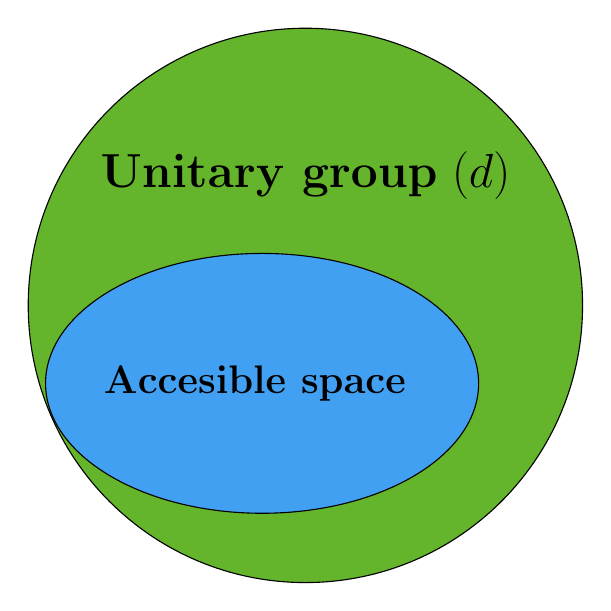
\begin{tikzpicture}[scale=1.1]
        \definecolor{circleColor}{RGB}{100,180,44}    % Green
        \definecolor{ellipseColor}{RGB}{65,160,241}   % Blue
        % Draw the circle
        \draw[fill=circleColor, draw=black] (0,0) circle (3.2cm);
        % Add text inside the circle
        \node at (0,1.5) {{\LARGE \textbf{Unitary group} $\calU(d)$}};
      
        % Draw the ellipse inside the circle
        \draw[fill=ellipseColor, draw=black] (-0.5,-0.9) ellipse (2.5cm and 1.5cm);
        % Add text inside the ellipse
        \node at (-0.5,-0.9) {{\LARGE \textbf{\Large Accesible space} $\bbU$}};
      \end{tikzpicture}
    \caption{ユニタリ群 $\calU(d)$ と量子回路の表現領域 $\bbU$}
    \label{fig:expressibility}
\end{figure}


\subsection{$p = 1$}
$p = 1$ のとき、$X$ として $\dyad{\bs{0}} := \dyad{0}\otn{n}$ を用いると、表現力は次のようになる。

\begin{align}
    \epsilon_{\bbU}^{(2,1)}(\dyad{\bs{0}}) &:= \norm{A^{(2)}(\dyad{\bs{0}})}_1\nonumber\\
    &= \Tr\abs{\int_{V\in\calU(d)} d\mu_{\Haar}(V)\,(V\dyad{\bs{0}}V\dg)\otn{2} - \int_{U\in\bbU} dU\,(U\dyad{\bs{0}}U\dg)\otn{2}}
\end{align}

トレースの第一項は以下のように計算される\cite{zhang2015matrix}。
\begin{align}
    \int_{V\in\calU(d)} d\mu_{\Haar}(V)\,(V\dyad{\bs{0}}V\dg)\otn{2} = \frac{\bbid_{d^2} + \SWAP}{d(d+1)},
\end{align}
ただし、$\SWAP := \sum_{i,j=1}^d \ket{ij}\bra{ji}$ である。


\subsection{$p = 2$}
$p = 2$ のとき、次の定理が成り立つ。
\begin{screen}
    \begin{theorem}
        表現力 $\epsilon_{\bbU}^{(t,2)}(X) = \norm{A^{(t)}(X)}_2$ は以下のようにフレームポテンシャルと呼ばれる量 $\calF$ によって表すことができる\cite{holmes2022connecting}。
        \begin{align}
            \epsilon_{\bbU}^{(t,2)}(X) &:= \sqrt{\calF_{\bbU}^{(t)}(X) - \calF_{\Haar}^{(t)}(X) }\\
            \calF_{\bbU}^{(t)}(X) &:= \int_{W\in\bbU}\int_{V\in\bbU} dWdV \Tr[WXW\dg (VXV\dg)\dg]^t\\
            \calF_{\Haar}^{(t)}(X)
            &:= \int_{W\in\calU(d)}\int_{V\in\calU(d)} d\mu_{\Haar}(W)d\mu_{\Haar}(V) \Tr[WXW\dg (VXV\dg)\dg]^t\nonumber\\
            &= \int_{V\in\calU(d)} d\mu_{\Haar}(V) \Tr[VX\dg V\dg X]^t
        \end{align}
        特に $t=2$ のとき、$\calF_{\calU(d)}^{(t)}(X)$ は、公式~\eqref{eq:haar-int-5} を用いて以下のように計算できる。
        \begin{align}
            \calF_{\Haar}^{(2)}(X) = \frac{\Tr[X^4] + \Tr[X^2]^2}{2^{2n} - 1} - \frac{2\Tr[X^2]\Tr[X]^2}{2^n(2^{2n} - 1)}
        \end{align}
    \end{theorem}
\end{screen}


\begin{proof}
    \begin{align}
        \qty{\epsilon_{\bbU}^{(t,2)}(X)}^2
        &:= \norm{A^{(t)}(X)}_2^2\\
        &:= \Tr\qty[A^{(t)}(X)\dg A^{(t)}(X)]\\
        &= \Tr\qty(\int_{V\in\calU(d)} d\mu_{\Haar}(V)\,(VX\dg V\dg)\otn{t} - \int_{U_1\in\bbU} dU_1\,(U_1X\dg U_1\dg)\otn{t}) \nonumber\\
        &\quad\; \times \qty(\int_{W\in\calU(d)} d\mu_{\Haar}(W)\,(WXW\dg)\otn{t} - \int_{U_2\in\bbU} dU_2\,(U_2XU_2\dg)\otn{t})\\
        &\overset{(1)}{=} \int_{V\in\calU(d)}\int_{W\in\calU(d)} d\mu_{\Haar}(V)d\mu_{\Haar}(W)\, \Tr[VX\dg V\dg WXW\dg]^t \nonumber\\
        &- \int_{V\in\calU(d)}\int_{U_2\in\bbU} d\mu_{\Haar}(V)dU_2\, \Tr[VX\dg V\dg U_2XU_2\dg]^t\nonumber\\
        &- \int_{U_1\in\bbU}\int_{W\in\calU(d)} dU_1d\mu_{\Haar}(W)\, \Tr[U_1X\dg U_1\dg WXW\dg]^t \nonumber\\
        &+ \int_{U_1\in\bbU}\int_{U_2\in\bbU} dU_1dU_2\, \Tr[U_1X\dg U_1\dg U_2XU_2\dg]^t\\
        &\overset{(2)}{=} \int_{V\in\calU(d)}\int_{W\in\calU(d)} d\mu_{\Haar}(V)d\mu_{\Haar}(W)\, \Tr[VX\dg V\dg X]^t \nonumber\\
        &- \int_{V\in\calU(d)}\int_{U_2\in\bbU} d\mu_{\Haar}(V)dU_2\, \Tr[VX\dg V\dg X]^t \nonumber\\
        &- \int_{U_1\in\bbU}\int_{W\in\calU(d)} dU_1d\mu_{\Haar}(W)\, \Tr[X\dg WXW\dg]^t \nonumber\\
        &+ \int_{U_1\in\bbU}\int_{U_2\in\bbU} dU_1dU_2\, \Tr[U_1X\dg U_1\dg U_2XU_2\dg]^t\\
        &\overset{(3)}{=} \int_{U_1\in\bbU}\int_{U_2\in\bbU} dU_1dU_2\, \Tr[U_1X\dg U_1\dg U_2XU_2\dg]^t \nonumber\\
        &- \int_{\calU(d)} d\mu_{\Haar}(V)\, \Tr[VX\dg V\dg X]^t\\
        &= \calF_{\bbU}^{(t)}(X) - \calF_{\Haar}^{(t)}(X)
    \end{align}
    等号(1)では、$A\otn{t} B\otn{t} = (AB)\otn{t}$ であることと、$\Tr[C\otn{t}] = \Tr[C]^t$ であることを用いた。等式(2)では、ハール分布の性質(両側不変性)を用いた。等式(3)では、$\int_{W\in\calU(d)} d\mu_{\Haar}(W) = \int_{U_{1,2}\in\bbU} dU_{1,2} = 1$ であることを用いた。
\end{proof}


\begin{screen}
    \begin{corollary}\label{cor:expressibility}
        $t = 2,\, X = \dyad{\bs{0}}$ のとき、表現力は次のように計算される\cite{holmes2022connecting}。
        \begin{align}\label{eq:expressibility-1}
            (\epsilon_{\bbU}^{(2,2)}(\dyad{\bs{0}}))^2 = \int_{W\in\bbU}\int_{V\in\bbU} dWdV |\bra{\bs{0}}W\dg V\ket{\bs{0}}|^4 - \frac{1}{2^{n-1}(2^n + 1)}
        \end{align}
    \end{corollary}
\end{screen}
式~\ref{eq:expressibility-1}の右辺の第一項をみると、これは対象となる量子回路から生成される2つの状態ベクトル $V\ket{\bs{0}},\,W\ket{\bs{0}}$ の内積の絶対値の4乗を積分(平均)したものであることがわかる。変分量子回路の表現力を数値計算で求める場合は、パラメーターをランダムにサンプリングして2つの状態ベクトルを生成し、それらの内積の絶対値の4乗を平均すればよい(モンテカルロ積分)。

\begin{proof}
    $X = \dyad{\bs{0}}$ のとき、$\calF_{\bbU}^{(2)}(\dyad{\bs{0}}),\, \calF_{\bbU}^{(2)}(\dyad{\bs{0}})$ は以下のように計算される。
    \begin{align}
        \calF_{\bbU}^{(2)}(\dyad{\bs{0}})
        &:= \int_{W\in\bbU}\int_{V\in\bbU} dWdV \Tr[W\dyad{\bs{0}}W\dg (V\dyad{\bs{0}}V\dg)\dg]^2\\
        &= \int_{W\in\bbU}\int_{V\in\bbU} dWdV |\bra{\bs{0}}W\dg V\ket{\bs{0}}|^4\\
        \calF_{\calU}^{(2)}(\dyad{\bs{0}})
        &:= \int_{W\in\calU}\int_{V\in\calU} d\mu_{\Haar}(W)d\mu_{\Haar}(V) \Tr[W\dyad{\bs{0}}W\dg (V\dyad{\bs{0}}V\dg)\dg]^2\\
        &= \int_{W\in\calU}\int_{V\in\calU} d\mu_{\Haar}(W)d\mu_{\Haar}(V) \Tr[(V\dg W)\dyad{\bs{0}} (V\dg W)\dg\dyad{\bs{0}}]^2\\
        &\overset{(1)}{=} \int_{W\in\calU}\int_{V\in\calU} d\mu_{\Haar}(W)d\mu_{\Haar}(V) \Tr[W\dyad{\bs{0}} W\dg\dyad{\bs{0}}]^2\\
        &\overset{(2)}{=} \int_{W\in\calU} d\mu_{\Haar}(W) \Tr[W\dyad{\bs{0}} W\dg\dyad{\bs{0}}]^2\\
        &= \int_{W\in\calU} d\mu_{\Haar}(W)\, \abs{\bra{\bs{0}}W\ket{\bs{0}}}^4\\
        &= \int_{W\in\calU} d\mu_{\Haar}(W)\, w_{\bs{0},\bs{0}}\,w_{\bs{0},\bs{0}}\,w^\ast_{\bs{0},\bs{0}}\,w^\ast_{\bs{0},\bs{0}}\\
        &\overset{(3)}{=} \frac{1}{2^{n-1}(2^n + 1)}
    \end{align}
    等号(1)では、ハール分布の性質(左不変性)を用いた。等号(2)では、$\int_{V\in\calU} d\mu_{\Haar}(V) = 1$ を用いた。等号(3)では、公式~\eqref{eq:haar-int-1} を用いた。
\end{proof}

% $p=2$ の場合、表現力は量子回路が生成するランダムな出力状態ベクトルの内積を積分することで計算できるが、$p=1$ の場合、表現力は密度演算子のテンソル積の積分が必要となる。したがって、$p=1$ の表現力は $p=2$ の表現力よりも計算コストが高い。


実際に系\ref{cor:expressibility}を用いて2つの具体的な量子回路に対して表現力 $(\epsilon_{\bbU}^{(2,2)}(\dyad{\bs{0}}))^2$ を計算してみる。
1つは、Tensor Product Ansatz (TPA) と呼ばれる回路であり、図~\ref{fig:tpa-alt}の左のような、2量子ビットゲートを持たない回路である。もう1つは、Alternating Layered Ansatz (ALT) と呼ばれる回路であり、図~\ref{fig:tpa-alt}の右のような、2量子ビットゲートを交互にずらして配置する量子回路である。

\begin{figure}[H]
    \centering
    \begin{tikzpicture}
        \node[scale=0.75]{
        \begin{quantikz}
            \lstick{$\ket{0}$}\slice{} & \gate{R_x} & \gate{R_y}\slice{1}& \gate{R_x} & \gate{R_y}\slice{2}& \gate{R_x} & \gate{R_y}\slice{3}& \meter{}\\
            \lstick{$\ket{0}$}      & \gate{R_x} & \gate{R_y}      & \gate{R_x} & \gate{R_y}      & \gate{R_x} & \gate{R_y}      & \meter{}\\
            \lstick{$\ket{0}$}      & \gate{R_x} & \gate{R_y}      & \gate{R_x} & \gate{R_y}      & \gate{R_x} & \gate{R_y}      & \meter{}\\
            \lstick{$\ket{0}$}      & \gate{R_x} & \gate{R_y}      & \gate{R_x} & \gate{R_y}      & \gate{R_x} & \gate{R_y}      & \meter{}\\
            \lstick{$\ket{0}$}      & \gate{R_x} & \gate{R_y}      & \gate{R_x} & \gate{R_y}      & \gate{R_x} & \gate{R_y}      & \meter{}\\
            \lstick{$\ket{0}$}      & \gate{R_x} & \gate{R_y}      & \gate{R_x} & \gate{R_y}      & \gate{R_x} & \gate{R_y}      & \meter{}
        \end{quantikz}
        \qquad
        \begin{quantikz}
            \lstick{$\ket{0}$}\slice{}&\gate{R_x}&\gate{R_y}&\ctrl{1}\slice{1}&\qw       &          &\qw\slice{2}&\gate{R_x}&\gate{R_y}&\ctrl{1}\slice{3}& \meter{}\\
            \lstick{$\ket{0}$}        &\gate{R_x}&\gate{R_y}&\targ{}          &\gate{R_x}&\gate{R_y}&\ctrl{1}    &\gate{R_x}&\gate{R_y}&\targ{}          & \meter{}\\
            \lstick{$\ket{0}$}        &\gate{R_x}&\gate{R_y}&\ctrl{1}         &\gate{R_x}&\gate{R_y}&\targ{}     &\gate{R_x}&\gate{R_y}&\ctrl{1}         & \meter{}\\
            \lstick{$\ket{0}$}        &\gate{R_x}&\gate{R_y}&\targ{}          &\gate{R_x}&\gate{R_y}&\ctrl{1}    &\gate{R_x}&\gate{R_y}&\targ{}          & \meter{}\\
            \lstick{$\ket{0}$}        &\gate{R_x}&\gate{R_y}&\ctrl{1}         &\gate{R_x}&\gate{R_y}&\targ{}     &\gate{R_x}&\gate{R_y}&\ctrl{1}         & \meter{}\\
            \lstick{$\ket{0}$}        &\gate{R_x}&\gate{R_y}&\targ{}          &\qw       &          &            &\gate{R_x}&\gate{R_y}&\targ{}          & \meter{}
        \end{quantikz}
        };
    \end{tikzpicture}
    \caption{6量子ビット3層の TPA(左)と ALT(右)}
    \label{fig:tpa-alt}
\end{figure}

TPA の表現力の2乗した値を各量子ビット数 $n$、各層数 $L$ について計算した結果を図~\ref{fig:circuit-exp}の左に示す。ALT の表現力の2乗した値を各量子ビット数 $n$、各層数 $L$ について計算した結果を図~\ref{fig:circuit-exp}の右に示す。
表現力は、全てのパラメーターを $5000$ 回ランダムにサンプリングして計算した。

\begin{figure}[H]
    \begin{minipage}[b]{0.5\columnwidth}
        \centering
        \includegraphics[width=8.5cm]{product-circuit-exp.pdf}
    \end{minipage}
    \hspace{0\columnwidth}
    \begin{minipage}[b]{0.5\columnwidth}
        \centering
        \includegraphics[width=8.5cm]{alt-circuit-exp.pdf}
    \end{minipage}
    \caption{TPA(左)と ALT(右)の表現力}
    \label{fig:circuit-exp}
\end{figure}

TPA はエンタングルメントを持たないため、一定以上の層数になると表現力がほとんど変化していない。一方、
ALT の総数を増やすほどエンタングルメントが増え、表現力が小さくなっていることがわかる。
